\documentclass[10pt,a4paper]{article}
\usepackage[utf8]{inputenc}
\usepackage{graphicx}
\title{Report of TweetoScope}
\author{Ilyas Moutawwakil, Hao Wang, Youness Laklouch}
\begin{document}
\maketitle

\section{Introduction}

In this project, we will create a java application displaying the trending hashtags in real-time from twitter using \textbf{Kafka} middle-ware to optimize the communication between different services. Then we want to deploy this application using \textbf{Docker} for containerization and \textbf{Kubernetes} for orchestration. Finally, we will use CI/CD to optimize the development process.

\section{Secrets and Git}

In this project, one needs a \textbf{BEARER\_TOKEN} from the \textbf{Twitter API} for developers.
Since its confidential and each member/user needs his own token to access the Twitter stream (using the same token simultaneously is impossible), we decided to make it an environment variable. The token in this case can be hidden, inferred from environment or stored in environment files. In all cases, it's not a good idea to push personal data to the Git repository or to hard code variables that change depending on the context (person, time,...).

\section{Architectural Choices}
\par
In the architecture that we've built, the stream of tweets is received from the twitter API then recorded in a \textbf{Kafka Topic : Tweets}. One single partition is used here because we only receive 1 percent of publicly available Tweets in real-time which are randomly sampled and also there is just one worker. 
\par
For the purpose of communicating between topics and finally sending Tweet information to the final Kafka consumer, our visualizer, we need to create a \textbf{Serializer} and \textbf{Deserializer} adapted for Tweet instances. Here, we use JSON-formatted string as information carrier with special date-time adapter.
\par
Then, we use Kafka Stream Services to filter out all the Tweets received from the previous topics based on certain rules like the language of Tweet, country where it has been posted, Tweet length, etc... This Kafka Service called \textbf{Filter} in the architecture, contains also : a hashtags extractor and a hashtags counter to rank the most frequent hashtags in real-time then send them to the next topic \textbf{Filtered-Tweets} where only count information is recorded.
\par
Finally, a visualizer to display the trending hashtag or topics on twitter is at the end of our solution.
\section{Risk Analysis}
In this section, we will discuss the impact of failure occurred on different component.
Different components work separately. So if any failure occurs, the whole application would hang instead of crashing : 
\begin{itemize}
    \item If the Stream crashes, the other two (Filter and Visualizer) would still be working but of course they won’t change anymore, since there are no more tweets coming their way
    \item If the Filter crashes, same thing the other
two would be running but the Visualizer would show erroneous results.
    \item If the Visualizer crashes, nothing would change in the other two.
\end{itemize}
\section{Risk mitigation using Kubernetes}
From what we can see in the figure below, when we delete the filter-deployment-694b4594b7 pod running on ic45, we see that Kubernetes is sticking
to the deployment we described and it creates a new filter-deployment-694b4594b7 pod running on ic22.

\begin{figure}[htbp]
\centering
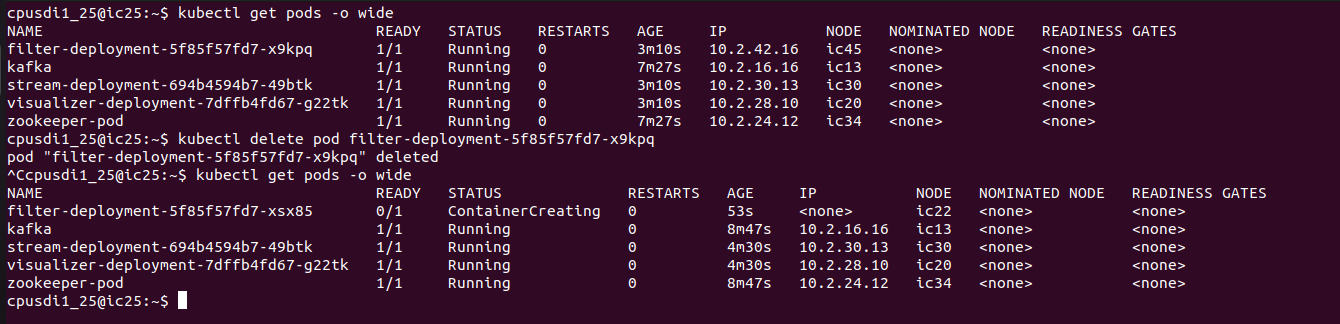
\includegraphics[scale = 0.3]{screenshot.png}
\end{figure}

\section{what we have learned by completing this project}
In this project we learned how hard to make my Kafka Application scalabale and fault tolerant using DevOps. We also learned that code is very fragile and instable and one little change in two developers environments can make it work on one machine but not on the other. And that's exactly the kind of questions we solved with CI/CD.

\section{Which parts were the most difficult and why ?}
The most difficult parts were the ones that deviated from what we did in Tutorials like X11 forwarding which we didn't know how to make it work but in the end we found a solution.  

\end{document}
